\documentclass[graphics,14pt]{beamer}
\geometry{papersize={338.7mm,190.5mm},margin={1.125cm,0.125cm}}
\usepackage[utf8]{inputenc}
\usepackage[brazil]{babel}
\usetheme{boxes}
\usepackage[sfdefault]{carlito}
\usepackage{natbib}
% -----------------------------------------------------------------------
% --- Slide Justificado -------------------------------------------------
\usepackage{ragged2e}
\usepackage{etoolbox}
\usepackage{scrextend} % ajustar texto para direita
\usepackage{soul}
\usepackage[normalem]{ulem}
\usepackage{cancel}
\usepackage{bm}
\usepackage{array}
\usepackage{wrapfig} 
\apptocmd{\frame}{}{\justifying}{} % Allow optional arguments after frame.
\usepackage{amsmath,mathtools}
\usepackage{verbatim}
% -----------------------------------------------------------------------
% separação entre colunas e linhas de tabelas
\setlength{\tabcolsep}{2pt}
\renewcommand{\arraystretch}{1}
% -----------------------------------------------------------------------
% --- Define a centralização de coluna com largura {|C{1 cm}|}
\newcolumntype{C}[1]{>{\centering\let\newline\\\arraybackslash\hspace{0pt}}m{#1}}
\newcolumntype{L}[1]{>{\raggedright\let\newline\\\arraybackslash\hspace{0pt}}m{#1}}
% -----------------------------------------------------------------------
\newcommand\litem[1]{\item{\bfseries #1 }}

% --- Letras e simbolos matemáticos -------------------------------------
%\usepackage[bbgreekl]{mathbbol}  % Pacote para repreentação de conjuntos com \mathbb{R} com letras gregas
%\usepackage{amsfonts}	% Pacote para repreentação de conjuntos com \mathbb{R}
%\usepackage{mathrsfs}	% Pacote para letras matemáticas
%\usepackage{amssymb} 	% diversos simbolos matematicos adicionais. Carrega automático com amsfonts
% ------------------------------------------------------------------------
\usepackage{multicol}
\usepackage{multimedia}
\usepackage[]{graphicx}
\usepackage[]{color}
\usepackage{geometry}
%\usepackage{media9}

\usepackage{tabularx}
%\usepackage{amsmath, amsthm, amssymb}
\usepackage{gensymb}

% ------------------------------------------------------------------------

% --- Esta definicao deve vir antes --------------------------------------
\usepackage{graphicx}			% Inclusão de gráficos
\usepackage{float}  
% ------------------------------------------------------------------------
\usefonttheme[onlymath]{serif}
\usepackage{hyperref}
 \usepackage{breakurl}
\usepackage{multirow}
\usepackage{subfig}
\usepackage{ragged2e}
%\captionsetup[subfigure]{labelformat=empty}
\usepackage{color}
\usepackage{colortbl}
\usepackage{textpos}
\usepackage{tikz}
\usetikzlibrary{calc}
%---------------
\usepackage{tabularx}
\usepackage{booktabs}
\usepackage{multimedia}
\usepackage[style=british]{csquotes}
\usepackage{listings}
%\usepackage[absolute,overlay]{textpos}
% ------------------------------------------------------------------------
\lstset{language=R,
	basicstyle=\large\ttfamily,
	stringstyle=\color{teal},
	otherkeywords={0,1,2,3,4,5,6,7,8,9},
	morekeywords={TRUE,FALSE},
	deletekeywords={data,frame,length,as,character},
	keywordstyle=\color{blue},
	commentstyle=\color{teal},
	showspaces=false,               % show spaces adding particular underscores
	showstringspaces=false,         % underline spaces within strings
	showtabs=false,                 % show tabs within strings adding particular underscores
%	frame=single,                   % adds a frame around the code
	tabsize=1,                      % sets default tabsize to 2 spaces
	captionpos=b,                   % sets the caption-position to bottom
	breaklines=true,                % sets automatic line breaking
	breakatwhitespace=false, 
}
% ------------------------------------------------------------------------
\pdfsuppresswarningpagegroup=1
\def\disciplina/{Estatística para Linguística}
% ------------------------------------------------------------------------
\tikzset{
	invisible/.style={opacity=0},
	visible on/.style={alt={#1{}{invisible}}},
	alt/.code args={<#1>#2#3}{%
		\alt<#1>{\pgfkeysalso{#2}}{\pgfkeysalso{#3}} % \pgfkeysalso doesn't change the path
	},
}
% ------------------------------------------------------------------------
\def\signed #1{{\leavevmode\unskip\nobreak\hfil\penalty50\hskip1em
		\hbox{}\nobreak\hfill #1%
		\parfillskip=0pt \finalhyphendemerits=0 \endgraf}}
\newsavebox\mybox
\newenvironment{aquote}[1]
{\savebox\mybox{#1}\begin{quote}}
	{\vspace*{1mm}\signed{\usebox\mybox}\end{quote}}
% ------------------------------------------------------------------------
% --- Desativando os botoes de navegacao ---------------------------------
\setbeamertemplate{navigation symbols}{}
% ------------------------------------------------------------------------
% --- Tela cheia ---------------------------------------------------------
\hypersetup{pdfpagemode=FullScreen}
% ------------------------------------------------------------------------
% --- Layout da pagina ---------------------------------------------------
\hypersetup{pdfpagelayout=SinglePage}
% ------------------------------------------------------------------------
% --- Relaxed footnotes --------------------------------------------------
\newcommand{\lfr}[1]{\let\thefootnote\relax\footnote{\hspace{0.6cm}\vspace{1.25cm} #1}}
% --- Pasta com as imagens -----------------------------------------------
\graphicspath{{Imagens/}}
% --- Define o cinza tema ------------------------------------------------
\definecolor{pcmggray}{rgb}{0.5, 0.5, 0.5}
% --- Define o estilo do titulo do frame ---------------------------------
\setbeamertemplate{frametitle}{ 
	\Huge{\bfseries{\insertframetitle\par}\vskip-18pt\hrulefill}
	\begin{tikzpicture}[remember picture,overlay]
	\node[xshift=0.65cm,yshift=-1.28 cm,opacity=1.0] at (current page.north west) {
\includegraphics[width=0.56cm]{00BAS_marcador_02.pdf}};
	\end{tikzpicture}
}
%\multicolbaselineskip = 1cm
 \columnsep = 1cm
% ------------------------------------------------------------------------
\setbeamercolor{frametitle}{fg=pcmggray,bg=white}
\setbeamerfont{structure}{size=\LARGE}
\setbeamerfont{itemize/enumerate body}{size=\LARGE}
\setbeamerfont{itemize/enumerate subbody}{size=\LARGE}
\setbeamerfont{normal text}{size=\LARGE}
\setbeamercolor{structure}{fg=black} % itemize, enumerate, etc
\setbeamercolor{section in toc}{fg=black} % TOC sections
\setbeamertemplate{bibliography item}{}
\setbeamerfont{bibliography item}{size=\normalsize}
\setbeamerfont{bibliography entry author}{size=\normalsize}
\setbeamerfont{bibliography entry title}{size=\normalsize,series=\bfseries}
\setbeamerfont{bibliography entry location}{size=\normalsize}
\setbeamerfont{bibliography entry note}{size=\normalsize}
\AtBeginDocument{\usebeamerfont{normal text}}
% --- Fundo da pagina de titulo ------------------------------------------
\setbeamertemplate{background} 
{
	\begin{tikzpicture}[remember picture, overlay]
	\node[xshift=5.75cm,yshift=-1.68cm,opacity=1.0] at (current page.north west) {
\includegraphics[width=11.49cm]{00BAS_titleleftupimage.pdf}};
	\node[xshift=16.93cm,yshift=-6.47cm,opacity=1.0] at (current page.north west) {
\includegraphics[width=18.0cm]{00BAS_ada_ufmg.pdf}};
	\node[xshift=28.35cm,yshift=-17.48cm,opacity=1.0] at (current page.north west) {
\includegraphics[width=11.04cm]{00BAS_titlerightdown.pdf}};
	\end{tikzpicture}
}
% ------------------------------------------------------------------------
\defbeamertemplate*{title page}{customized}[1][]
{
	\begin{center}
	\vspace{-1.5cm}
	\usebeamerfont{title}\LARGE{\textbf{\inserttitle}}\par
	\vspace{9cm}
	\usebeamerfont{subtitle}\huge{\textbf{\insertsubtitle}}\par
	\vspace{2cm}
	\usebeamerfont{author}\textbf{\insertauthor}\par
	\end{center}
	\vfill
}
\title{Laboratório de Fonologia}
\subtitle{\disciplina/}
\author[Silva, A. P.]{Prof. Dr. Adelino Pinheiro Silva}
\date{\today}
% =======================================================================
% INICIO DO CONTEUDO PRINCIPAL
% =======================================================================
\begin{document}
 \frame{\titlepage}
% =======================================================================
% ---- Fundo da demais paginas ------------------------------------------
\setbeamertemplate{background} 
{
	\begin{tikzpicture}[remember picture, overlay]
	\node[xshift=1.14cm,yshift=-18.08cm,opacity=1.0] at (current page.north west) {
\includegraphics[width=1.58cm]{00BAS_fale_logo.pdf}};
	\node[xshift=28.97cm,yshift=-18.2cm,opacity=1.0] at (current page.north west) {
\includegraphics[width=9.8cm]{00BAS_regularrightdown.pdf}};
	\end{tikzpicture}
	\put(880,-20){\Large{\insertframenumber \hspace{2pt} de \inserttotalframenumber}}
%	\begin{textblock}{2cm}(150pt,1pt)
%		\normalsize \insertframenumber de \inserttotalframenumber
%	\end{textblock}
%	\normalsize \insertframenumber de \inserttotalframenumber
}
% ==== Sumário ==========================================================
\section{Introdução}
\begin{frame}[t]
    \frametitle{Sumário}
    \begin{multicols}{2}
	    \tableofcontents
    \end{multicols}

\end{frame}
% ========================================================================

% ========================================================================
\AtBeginSection[]
{
  \begin{frame}[t]
    \frametitle{Assunto}
    \begin{multicols}{2}
    	\tableofcontents[currentsection]
    \end{multicols}
  \end{frame}
}
% =======================================================================

% ==== AULA 01 ==========================================================
\section{Introdução}
% ------------------------------------------------------------------------
\begin{frame}
	\frametitle{In a hole in the ground there lived a...}

	Por que estudar estatística?
	\begin{itemize}
		\item[-] Compreender \textbf{fatores} que afetam um resultado.
		\item[-] Julgar de forma crítica as informações recebidas.
		\item[-] Argumentar estatisticamente.
	\end{itemize}
	
	\vspace{2cm}
		
	O que é estatística \citep{Agresti2018}?
	\begin{itemize}
		\item[-] Conjunto de métodos para se \textbf{obter} e \textbf{analisar} dados.
		\item[-] Metodologia baseada na \textbf{ocorrência} \\ para realizar \textbf{previsão}.
	\end{itemize}

	\begin{tikzpicture}[remember picture,overlay]
		\node[xshift=10.5cm,yshift=1.50cm,opacity=1.0] at (current page.center) {
\includegraphics[width=12cm]{est_01_desvio_padrao.jpg}};
	\end{tikzpicture}
	\vfill
	\lfr{Imagem: \url{https://i.pinimg.com/originals/48/fb/95/48fb9570a8413fe83053df7c3599e7eb.jpg}}
\end{frame} 
% ------------------------------------------------------------------------
\begin{frame}
	\frametitle{I Have the High Ground}

	Alguns termos para começar
	\begin{itemize}
		\item[-] \textbf{Dado}: Observação obtida sobre o objeto de interesse.
		\item[-] \textbf{Observação}: Medida, ou informação coletada (sujeita a ruído e erros).
		\item[-] \textbf{Base de dados}: Conjunto de dados, e.g., \textit{general social survey}.
		\item[-] \textbf{População}: Conjunto total dos elementos (desconhecido, inacessível).
		\item[-] \textbf{Amostra}: subconjunto da população, dados (medidas) coletados.
		\item[-] \textbf{Parâmetro}: Fator (resumo) numérico da população (dica: letras gregas).
		\item[-] \textbf{Estatística}: Valor obtido da amostra !!!!!
		\item[-] \textbf{Ferramental}: R-studio
	\end{itemize}
	\begin{tikzpicture}[remember picture,overlay]
	\node[xshift=7.5cm,yshift=-4.0cm,opacity=1.0] at (current page.center) {
\includegraphics[width=12cm]{R-studio-logo.png}};
	\end{tikzpicture}
	\vfill
	\lfr{Imagem: \url{https://www.python.org/static/community_logos/python-logo-generic.svg}}
\end{frame}  
% ------------------------------------------------------------------------
\begin{frame}
\frametitle{I Have the High Ground}
	\begin{tikzpicture}[remember picture,overlay]
	\node[xshift=0cm,yshift=0.0cm,opacity=1.0] at (current page.center) {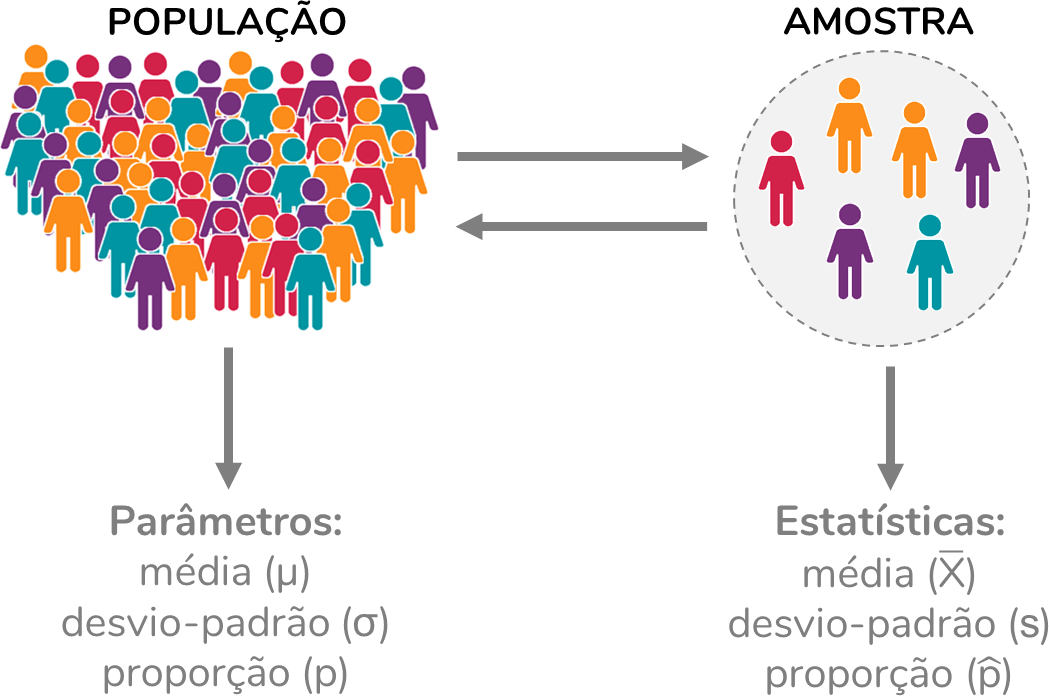
\includegraphics[width=22cm]{amostra-populacao_v0.png}};
	\end{tikzpicture}
	\vfill
	\lfr{Imagem: \url{https://fernandafperes.com.br/intervalo-de-confianca/}}
\end{frame}
% ------------------------------------------------------------------------
\begin{frame}
\frametitle{Medida e amostra}
	Maneiras de extrair informações de interesse.\\
	\begin{itemize}
		\item[-] \textbf{Variável aleatória}: Característica que pode variar com os elementos da população ou amostra.
		
		\item[-] \textbf{Escala de medição}: Extensão onde a variável aleatória pode ser medida. Exemplos:
			\begin{itemize}
				\item[-] Categóricas: (cara, coroa), (derrota, empate, vitória); ou
				\item[-] Quantitativas: $\{ x \in \mathbb{R} | 0 \leq x \leq 1\} $, $[0,1]$
			\end{itemize}
	\end{itemize}


	Se caracteriza a variável aleatória como um resultado de uma experiência aleatória, que pode ser classificada como:
	\begin{itemize}
		\item[-] \textbf{Categóricas}: valores aceitos dentro de um limite de categorias (qualitativos?).
		\item[-] \textbf{Quantitativas}: valores numéricos de qualquer conjunto, e.g., $\mathbb{N}$, $\mathbb{R}$, $\mathbb{C}$
	\end{itemize}
	\vfill
	\lfr{Definição formal de variável aleatória: $X:\Omega \to \mathbb{R} \Leftrightarrow \{ \omega: X(\omega) \leq x \} \in \mathcal{F}, \forall x \in \mathbb{R} $}
\end{frame}

% ------------------------------------------------------------------------
\begin{frame}
\frametitle{Medida e amostra}
	Escalas:.\\
	\begin{itemize}
		\item[-] \textbf{Intervalar}: delimitação numérica.
		\item[-] \textbf{Nominal}: Nomes/categorias ``não ordenáveis'', e.g., preferência de cores;
		\item[-] \textbf{Ordenáveis}: Nomes/categorias que podem ser ordenadas em níveis, e.g., expectativa do curso (baixá, sem expectativa, alta).	
	\end{itemize}
	
	Detalhe: Em escalas categóricas é muito difícil garantir uma homogeneidade dos intervalos, i.e., se os intervalos das categorias possuem escalas de mesmo tamanho.
	
	

\end{frame}
% ------------------------------------------------------------------------
\begin{frame}
\frametitle{Variáveis estatísticas}
	\begin{columns}[T] % align columns
		\begin{column}{.40\textwidth}
			\begin{itemize}
				\item[-] \textbf{Amostra aleatória simples}: todas amostras de mesmo tamanho possem a mesma ``chance''. Seria um retrato da população(?).
				\item[-] \textbf{Métodos de amostragem, \textit{sample survey}}: Sistemática, estratificada, grupo (\textit{cluster}), multiestágios.
				\item[-] \textbf{Amostra enviesada}: alunos de uma sala de aula (?).
			\end{itemize}
		\end{column}%
		\hfill%
		\begin{column}{.48\textwidth}	
		
		\end{column}%
	\end{columns}
	\begin{tikzpicture}[remember picture,overlay]
	\node[xshift=7cm,yshift=0.0cm,opacity=1.0] at (current page.center) {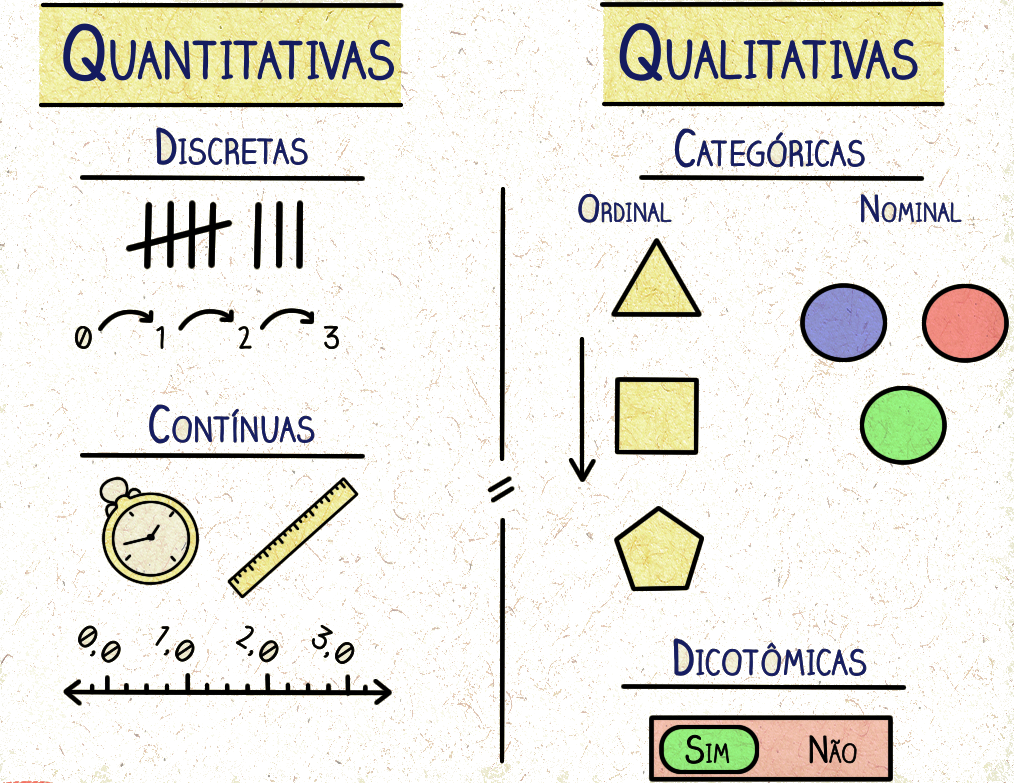
\includegraphics[width=18cm]{variaveis-estatisticas.png}};
	\end{tikzpicture}
	\vfill
	\lfr{Adaptado de \url{https://artemetabolica.blogspot.com/2015/12/bioestatistica-1-variaveis.html}}
\end{frame}
% ------------------------------------------------------------------------
\begin{frame}
\frametitle{Estudo experimental}
	\textbf{Experimento:} Controlar variáveis independentes e observar a variação de variáveis dependentes para dar suporte ou refutar uma hipótese.\\
	\begin{itemize}
		\item[-] Compara ``tratamentos''.
		\item[-] Unidades de testes.
		\item[-] Grupos, pelo menos, ``controle'' e ``tratamento''.
		\item[-] Variáveis estranhas (predatórias).
	\end{itemize}
%	Efeitos do teste: principal e interativo\\
%	Regressão analítica
	Problemas experimentais\\
		\begin{itemize}
		\item[-] Variação do instrumento (ou pessoa que conduz parte dele).
		\item[-] Regressão analítica.
		\item[-] Viés de seleção.
		\item[-] Perda de unidade
	\end{itemize}	
	\begin{tikzpicture}[remember picture,overlay]
	\node[xshift=12cm,yshift=-4.0cm,opacity=1.0] at (current page.center) {
\includegraphics[width=10cm]{Experimento-criancas.jpg}};
	\end{tikzpicture}

	\vfill
	\lfr{ \url{https://br.freepik.com/vetores-premium/}}
\end{frame}
% ------------------------------------------------------------------------
\begin{frame}
\frametitle{Estudo experimental}
	\vspace{-1.5cm}
	Efeitos do teste: principal e interativo\\
	\vspace{1cm}
	\textbf{Soluções para experimentos}:\\
	\begin{itemize}
		\item[-] Aleatorização.
		\item[-] Emparelhamento.
		\item[-] controle estatístico.
		\item[-] Planejamento.
		\item[-] Medições a \textit{posteriori}.
	\end{itemize}
	\begin{tikzpicture}[remember picture,overlay]
	\node[xshift=12cm,yshift=-4.0cm,opacity=1.0] at (current page.center) {
\includegraphics[width=10cm]{Experimento-criancas.jpg}};
	\end{tikzpicture}
	
	\vfill
	\lfr{ \url{https://br.freepik.com/vetores-premium/}}
	%	Efeitos do teste: pr
\end{frame}
% ------------------------------------------------------------------------
\begin{frame}
\frametitle{Estudo de Observação}
	\begin{tikzpicture}[remember picture,overlay]
\node[xshift=5cm,yshift=-2.5cm,opacity=1.0] at (current page.center) {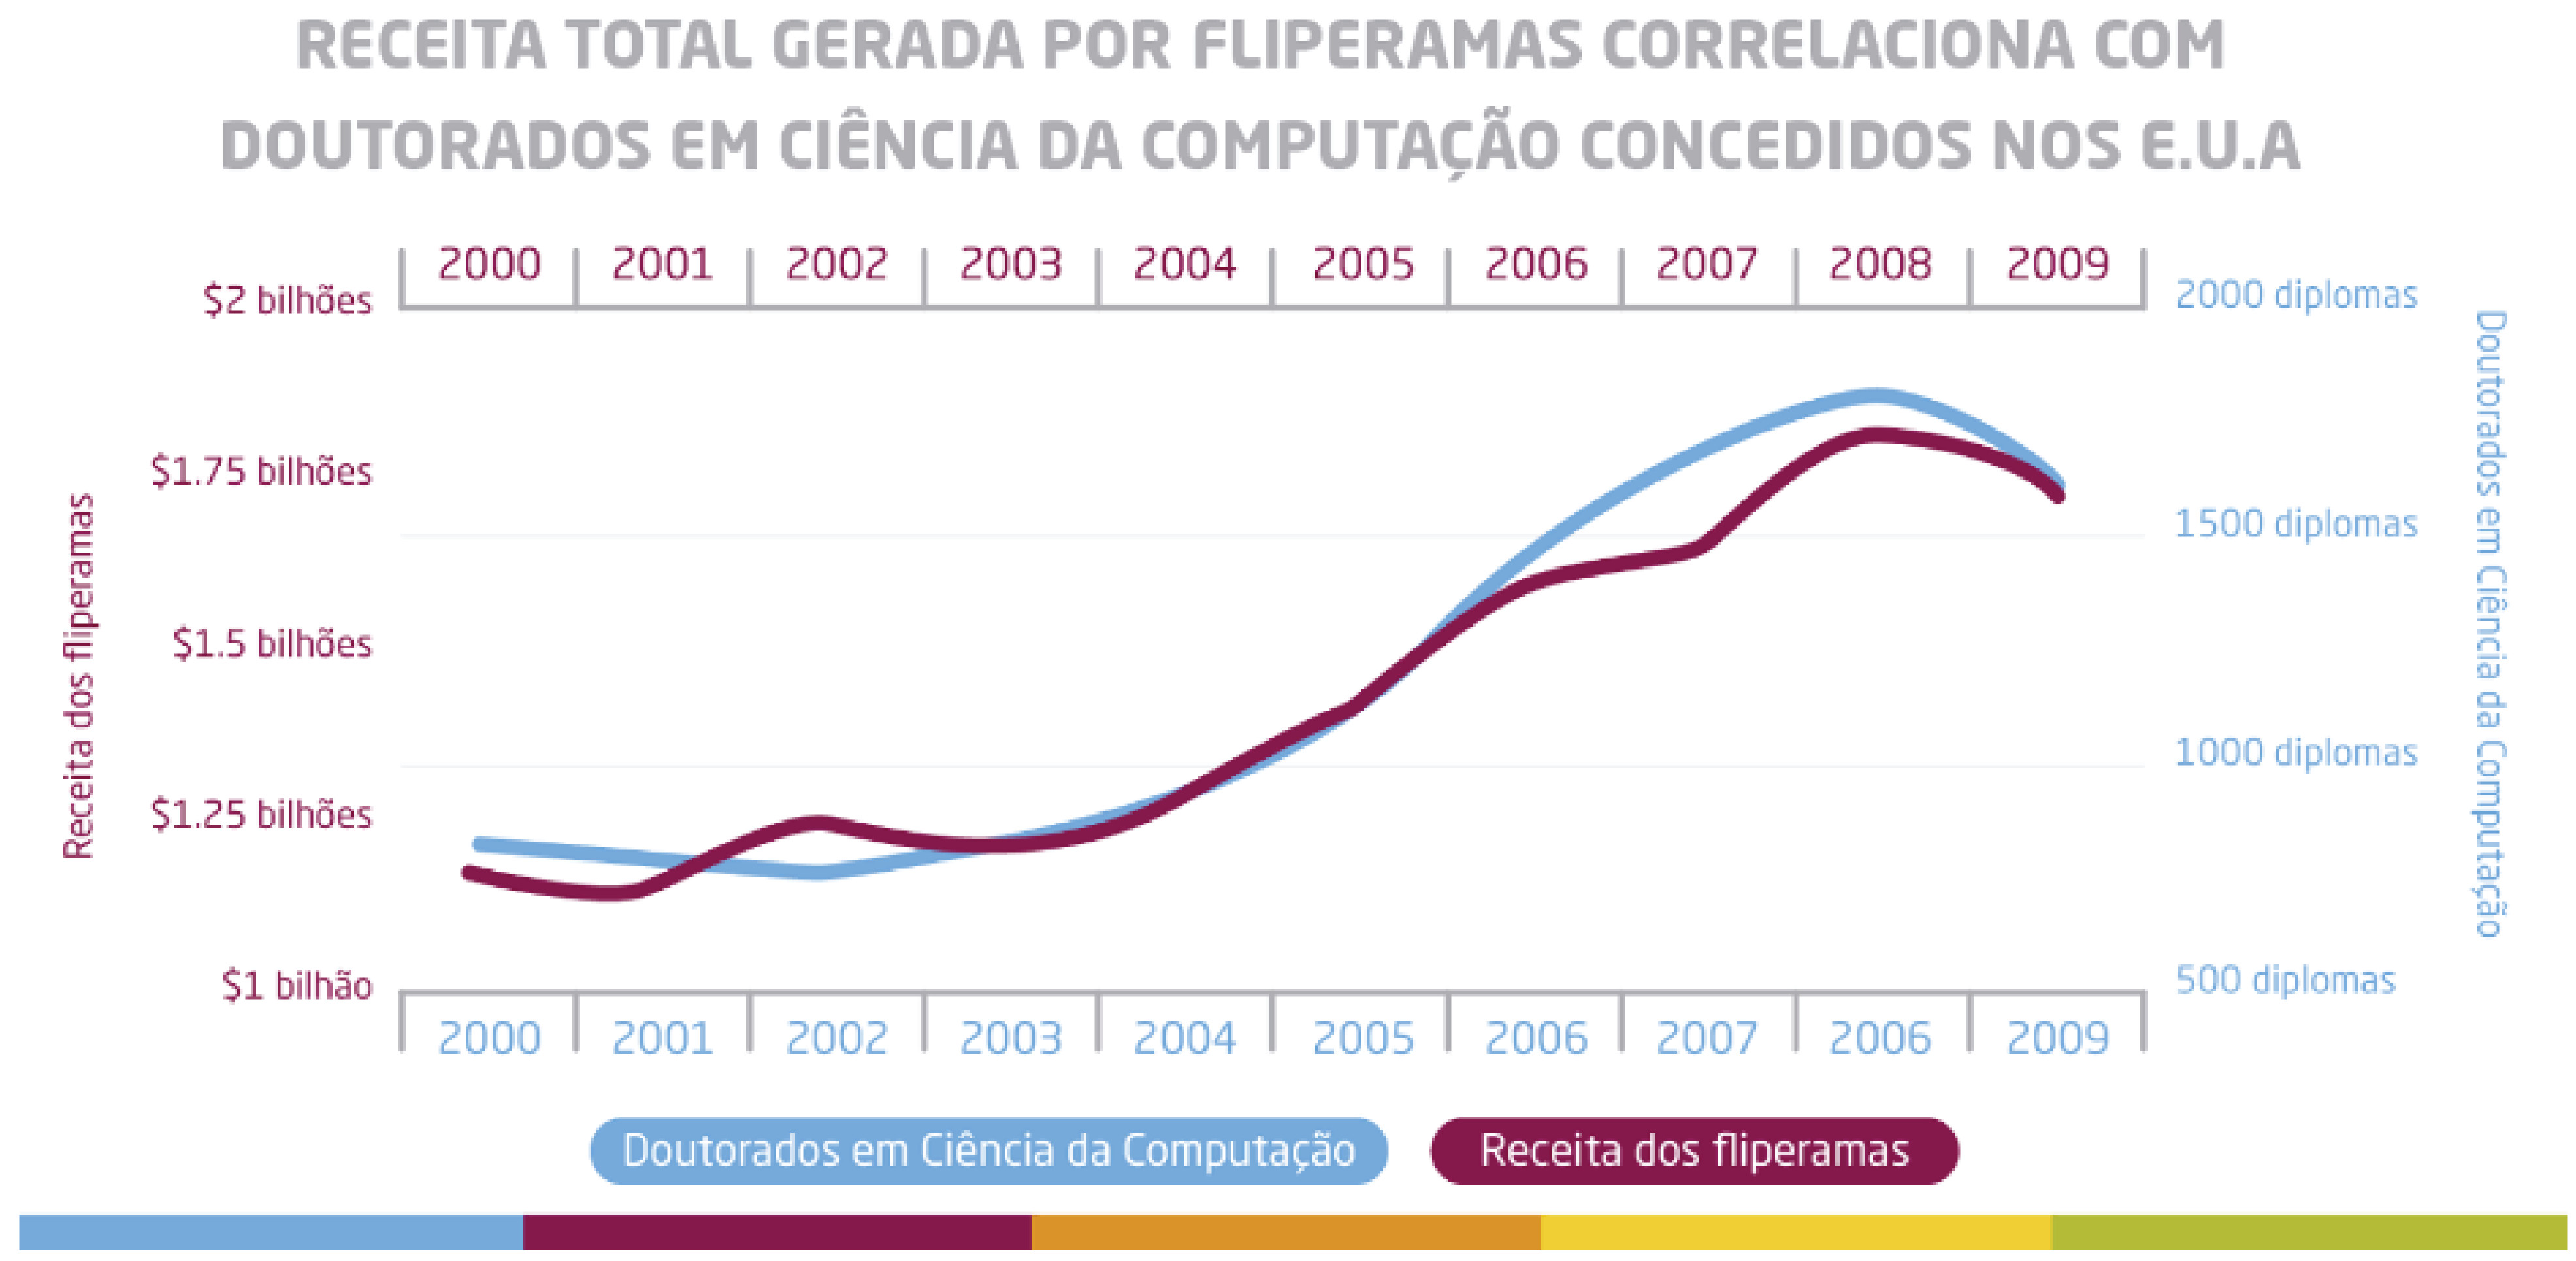
\includegraphics[width=23cm]{exemplo-de-correlacao-sem-causalidade.png}};
\end{tikzpicture}
\vspace{-2.5cm}
	\begin{itemize}
		\item[-] Sem manipulação do objeto de estudo.
		\item[-] Grupos desbalanceados, difícil de realizar uma comparação adequada.
		\item[-] \textbf{Não permite estabelecer causa e efeito}.
		\item[-] Pode indicar uma relação \\ entre variáveis.
		\item[-] Uma variável não medida \\ pode ser responsável \\ pelo padrão observado.
	\end{itemize}
%	\begin{tikzpicture}[remember picture,overlay]
%	\node[xshift=12cm,yshift=-4.0cm,opacity=1.0] at (current page.center) {\includegraphics[width=12cm]{exemplo-de-correlação-sem-causalidade.jpg}};
%	\end{tikzpicture}

	\vfill
	\lfr{ \url{http://blog.bravi.com.br/wp-content/uploads/2017/10}}
\end{frame}
% ------------------------------------------------------------------------
\begin{frame}
\frametitle{Variabilidade amostral e viés}
\vspace{-2cm}
	\textbf{Erro de amostragem:} erro ocorrido ao utilizar uma estatística da amostra para predizer um parâmetro da população. Exemplo: Erro da pesquisa eleitoral com n = 1000 de + ou - 3\%. \\
	\vspace{1cm}
	Viés: erro quando a amostra é enviesada, e.g., voluntários ou respostas de carta.\\
	\begin{itemize}
		\item[-] \textbf{Viés de resposta} ocorre quando a pergunta é confusa, e.g., referendo do desarmamento;
		\item[-] \textbf{viés de falha de dados} apenas uma fatia da amostra responde.
	\end{itemize}
	\vfill
\end{frame}
% ------------------------------------------------------------------------
	\begin{frame}
	\frametitle{Fim da introdução - Dever de casa}
		\textbf{Exercícios do livro \cite{Agresti2018}:}
		\begin{itemize}
			\item[-] Capítulo 1: 1.1, 1.3, 1.5-1.8, 1.14, 1.16;
			\item[-] Capítulo 2: 2.2-2.10,2.27, 2.35-2.37,2.39
		\end{itemize}
		\textbf{Preparação do terreno}
		\begin{itemize}
			\item[-] Instalar o R-studio.
		\end{itemize}	

	\end{frame}   
% ------------------------------------------------------------------------
\section{Estatística Descritiva}
% ------------------------------------------------------------------------
\begin{frame}[t,fragile=singleslide]
\frametitle{Estatística descritiva}
	Primeiro passo para entender os dados coletados\\
	Facilitar a assimilação de informação\\
	Medidas de:
	\begin{itemize}
		\item[-] tendência central (média), variabilidade, associação, etc...
	\end{itemize}
	Análise e regressão: predizer uma variável a partir de outras.\\
	\vspace{1.0cm}
	Um pouco de código R para tratar com dados
	\begin{lstlisting}
	data_lemas <- read.table("../Dados/lexporbr_alfa_lemas_txt.txt", header = TRUE, 
							sep = "\t",dec = ",",quote = "\"")
	head(data_lemas)
	dim(data_lemas)
	summary(data_lemas)
	\end{lstlisting}
	\vspace{1.0cm}	
	Dados de \href{https://www.lexicodoportugues.com/}{Corpus Léxico do português}
	\vfill
	\lfr{Dados: \url{https://www.lexicodoportugues.com/downloads/lexporbr_alfa_lemas_txt.txt}}

\end{frame}
% ------------------------------------------------------------------------
\begin{frame}[t,fragile=singleslide]
\frametitle{Tabelas e gráficos}
	Extraindo o cabeçalho dos dados
	\begin{lstlisting}
	> head(data_lemas)
	\end{lstlisting}
	Gera a saída:
	\begin{addmargin}[2.45cm]{0em}
		\normalsize 
		\begin{verbatim}
		id ortografia cat_gram inf_gram freq_orto freq_orto.M log10_freq_orto zipf_escala nb_letras
		1  1          o     gram      det   4364416   139093.06          6.6399      8.1433         1
		2  2         de     gram      prp   2553292    81372.90          6.4071      7.9105         2
		3  3          ,     gram       pu   2133025    67979.08          6.3290      7.8324         1
		4  4          .     gram       pu   1603184    51093.15          6.2050      7.7084         1
		5  5         em     gram      prp   1044260    33280.36          6.0188      7.5222         2
		6  6          e     gram       kc    667736    21280.61          5.8246      7.3280         1
		\end{verbatim}
	\end{addmargin}
	A dimensionalidade dos dados, onde cada linha indica uma medição com as colunas indicando as informações\\
	\begin{lstlisting}
	> dim(data_lemas)
	\end{lstlisting}
	Que é um total de 169.606 linhas com 9 colunas
	\begin{addmargin}[2cm]{0em}
	\normalsize 
	\begin{verbatim}
		[1] 169606      9
	\end{verbatim}
	\end{addmargin}

\end{frame}
% ------------------------------------------------------------------------
\begin{frame}[t,fragile=singleslide]
	\frametitle{Tabelas de contingência}
	Construindo uma tabela
	\begin{lstlisting}
	> tab <- table(data_lemas$cat_gram, data_lemas$nb_letras)
	\end{lstlisting}
	\vspace{2.0cm}

	\begin{addmargin}[2cm]{0em}
		\normalsize 
		\begin{verbatim}
		         1     2     3     4     5     6     7     8     9    10    11    12    13
		adj      3    41   355   699  1061  1490  2320  2817  3117  3106  2672  2099  1575
		adv      2    15    31    57    80    96   109   115   148   235   255   313   330
		gram    56    60    96    75    75    47    22    12    14     8     1     2     0
		nom     57   500  1517  3375  4992  5924  7396  7504  7397  6719  5912  4278  3151
		num     11   275  2045  5678 14704 11792  8534  6535  3553   913   941  1630   657
		ver      1    11    51   175  1037  1796  2099  2442  2115  1678  1123   815   475
		\end{verbatim}
	\end{addmargin}
	
\end{frame}
% ------------------------------------------------------------------------
\begin{frame}[t,fragile=singleslide]
\frametitle{Histograma}
	Histograma em uma figura PNG...
	\begin{lstlisting}
	png(file = ""../Imagens/histograma.png",width = 864, height = 486, units = "px")
	hist(data_lemas$nb_letras,main="Histograma do numero de letras em cada ocorrencia",
	breaks=40,xlab = "numero de letras", ylab="Ocorrencias",col = "blue2",
	border="white")
	dev.off()
	\end{lstlisting}
	\begin{tikzpicture}[remember picture,overlay]
	\node[xshift=6cm,yshift=-2.75cm,opacity=1.0] at (current page.center) {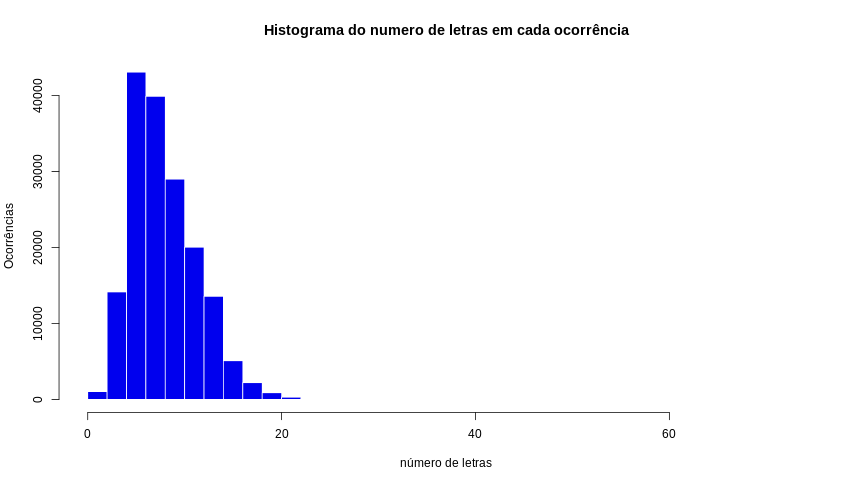
\includegraphics[width=24cm]{histograma.png}};
	\end{tikzpicture}
	\vfill
\end{frame}
% ------------------------------------------------------------------------
\begin{frame}[t,fragile=singleslide]
\frametitle{Diagrama de caixa}
	Diagrama de caixa (\textit{boxplot}) em uma figura PNG...
	\begin{lstlisting}
	png(file = "../Imagens/Box_plot.png",width = 864, height = 486, units = "px")
	boxplot(data_lemas$nb_letras ~ cat_gram, data = data_lemas, ylab = "Numero de letras", 
	col = "blue2", border="black")
	dev.off()
	\end{lstlisting}
	\begin{tikzpicture}[remember picture,overlay]
	\node[xshift=4cm,yshift=-2.75cm,opacity=1.0] at (current page.center) {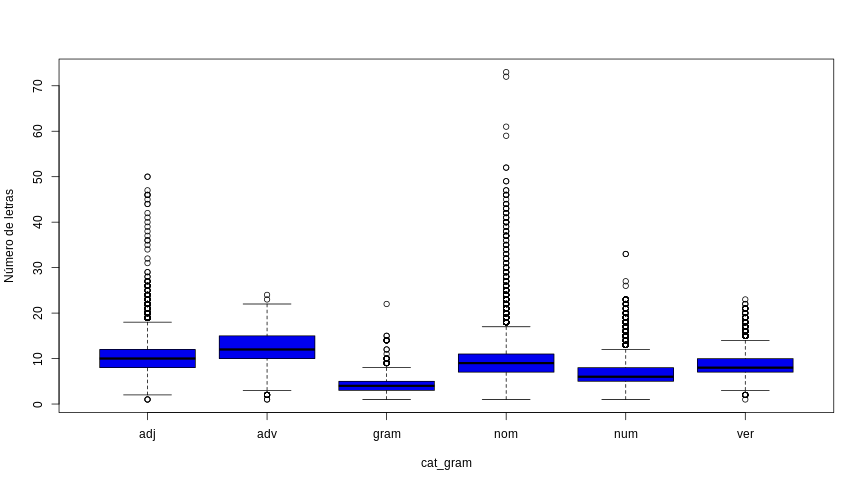
\includegraphics[width=24cm]{Box_plot.png}};
	\end{tikzpicture}
	\vfill
\end{frame}
% ------------------------------------------------------------------------
\begin{frame}[t,fragile=singleslide]
\frametitle{Diagrama ramo e folha}
	Apenas do primeiro ao 300º elemento
	\begin{lstlisting}
	> tab <- stem(data_lemas$nb_letras[1:300])
	\end{lstlisting}
	\vspace{2.0cm}
	
	\begin{addmargin}[2cm]{0em}
		\normalsize 
		\begin{verbatim}
		  The decimal point is at the |
		
		 1 | 0000000000000000000
		 2 | 0000000000000000000
		 3 | 0000000000000000000000000000000000000
		 4 | 00000000000000000000000000000000000000000
		 5 | 00000000000000000000000000000000000000000000000000000000000000
		 6 | 00000000000000000000000000000000000000000000
		 7 | 000000000000000000000000000000000000000
		 8 | 0000000000000000000000
		 9 | 000000000
		10 | 0000000
		11 | 
		12 | 
		13 | 0
		\end{verbatim}
	\end{addmargin}

\end{frame}
% ------------------------------------------------------------------------
\begin{frame}[t,fragile=singleslide]
\frametitle{Medidas de tendência central}
	\begin{tikzpicture}[remember picture,overlay]
	\node[xshift=7cm,yshift=-3.0cm,opacity=1.0] at (current page.center) {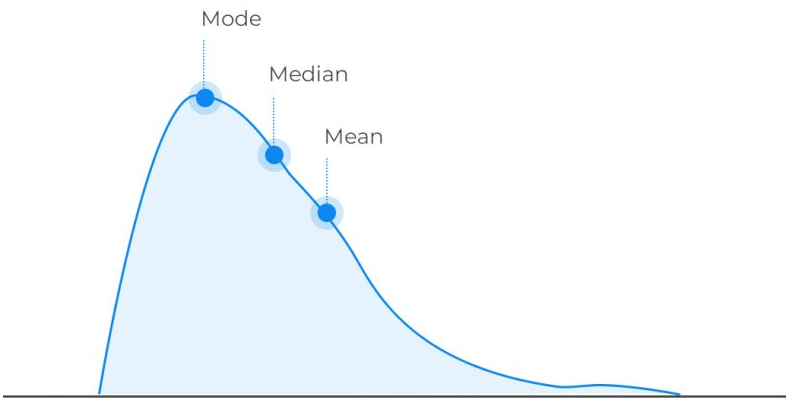
\includegraphics[width=18cm]{tendencia-central.png}};
	\end{tikzpicture}
	\vspace{-1.5cm}
	\begin{itemize}
		\item[-] Média
			\begin{itemize}
				\item[-] Aritmética: problema que \textit{outliers} podem alavancar.
				\item[-] Truncada (\textit{winsorized})
				\item[-] Ponderada
			\end{itemize}
		\item[-] Mediana: menos problemas com \textit{outliers}.
		\item[-] Moda: bem indicada para variáveis categóricas.
		\item[-] Tri-média: utiliza quartis.
	\end{itemize}
	
	
	\vfill
	\lfr{Adaptado de: \url{https://analystprep.com/cfa-level-1-exam/wp-content/uploads/2020/01/page-45-1024x673.jpg}}
\end{frame}
% ------------------------------------------------------------------------
\begin{frame}[t,fragile=singleslide]
\frametitle{Medidas de dispersão}
	\begin{tikzpicture}[remember picture,overlay]
	\node[xshift=6cm,yshift=-1.0cm,opacity=1.0] at (current page.center) {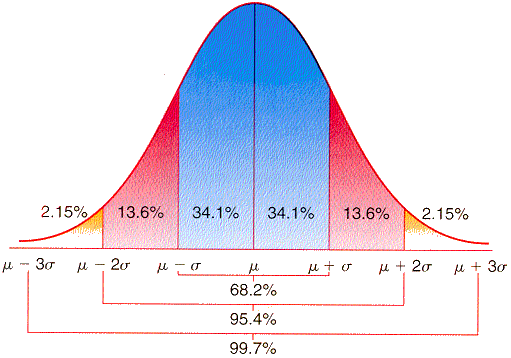
\includegraphics[width=18cm]{desvio-sigma.png}};
	\end{tikzpicture}
	\vspace{-1.5cm}
	\begin{itemize}
		\item[-] \textit{Range}, alcance, diferença entre mínimo e máximo.
		\item[-] desvios
		\begin{itemize}
			\item[-] variância e desvio padrão.
			\item[-] Soma dos desvios quadrados.
		\end{itemize}
		\item[-] Distância inter-percentis.
		\item[-] \textbf{Erro padrão}: desvio padrão da média
		\item[-] Regra do $\sigma$: 
		\begin{itemize}
			\item[-] $0,67\sigma \rightarrow 50\%$
			\item[-] $1\sigma \rightarrow 68,3\%$
			\item[-] $1,96\sigma \rightarrow 95\%$
			\item[-] $2\sigma \rightarrow 95,4\%$
			\item[-] $3\sigma \rightarrow 99,7\%$			
		\end{itemize}
	\end{itemize}

	\vfill
	\lfr{Adaptado de: \url{https://civilblog.org/2014/05/11/what-is-standard-deviation-and-how-to-calculate-it-with-an-example-calculation/}}
\end{frame}
% ------------------------------------------------------------------------
\begin{frame}[t,fragile=singleslide]
\frametitle{Achatamento(curtose) e (As)simetria}
	Mais medidas de caracterização dos dados
	\begin{lstlisting}
	library(moments)
	curt_data <- kurtosis(vec_n_letras_sel)
	assi_data <- skewness(vec_n_letras_sel)
	\end{lstlisting}
	\vspace{2.0cm}
	
	\begin{tikzpicture}[remember picture,overlay]
	\node[xshift=-4.5cm,yshift=-3.75cm,opacity=1.0] at (current page.center) {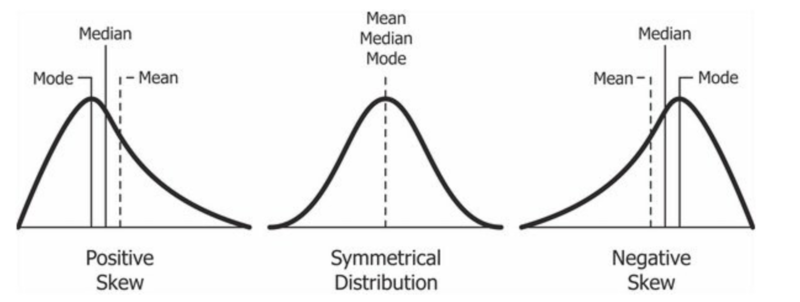
\includegraphics[width=20cm]{different_skewness.png}};
	\end{tikzpicture}
	\begin{tikzpicture}[remember picture,overlay]
	\node[xshift=9.5cm,yshift=2cm,opacity=1.0] at (current page.center) {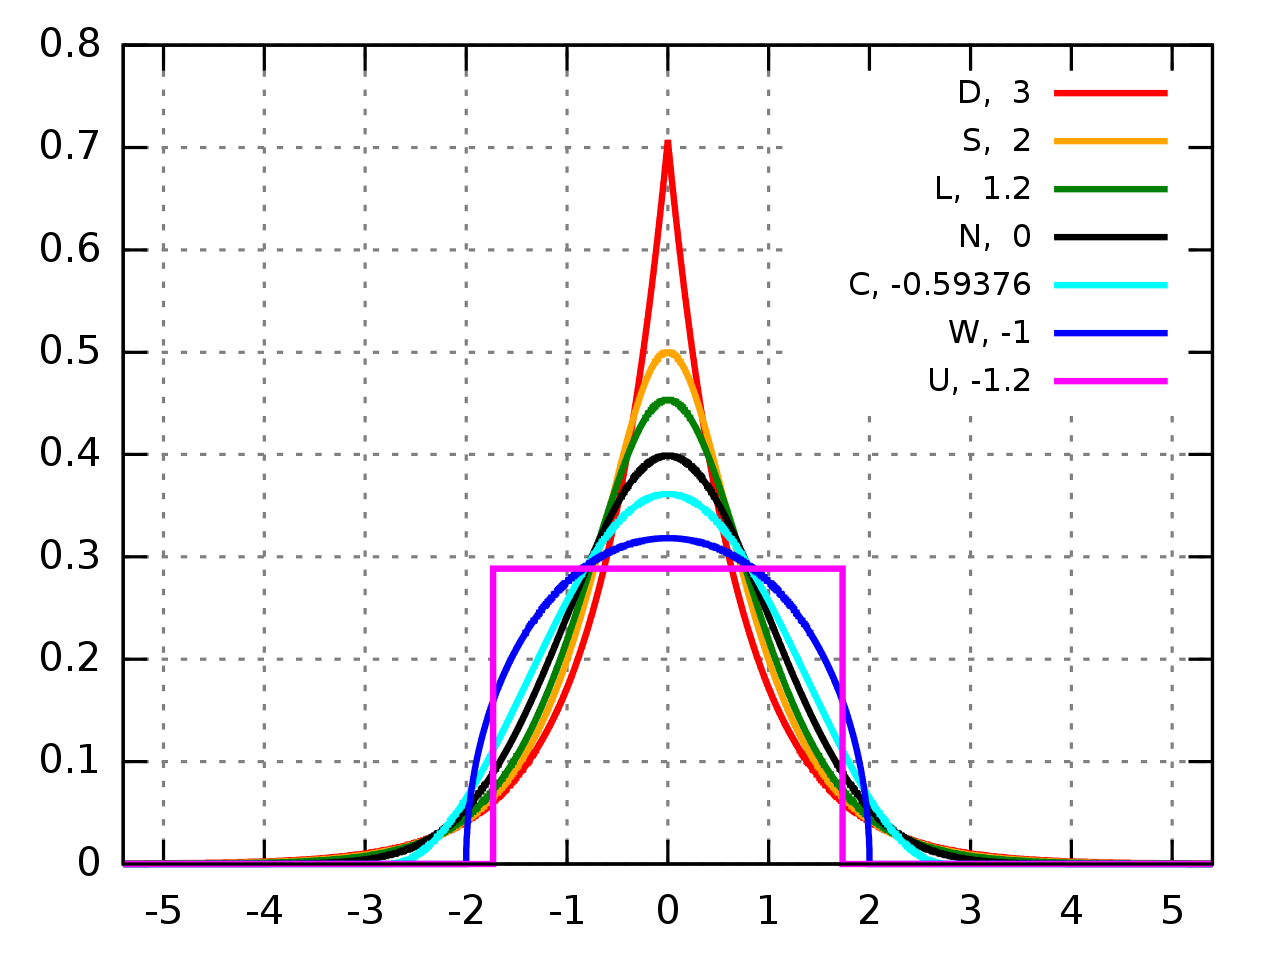
\includegraphics[width=12cm]{curtose_pdfs.png}};
	\end{tikzpicture}
	\vfill
\lfr{\url{https://en.wikipedia.org/wiki/Kurtosis} e \url{https://en.wikipedia.org/wiki/}}

\end{frame}
% ------------------------------------------------------------------------
\begin{frame}[t,fragile=singleslide]
\frametitle{Exemplos de Estatísticas}
	\begin{tikzpicture}[remember picture,overlay]
	\node[xshift=7.5cm,yshift=-4cm,opacity=1.0] at (current page.center) {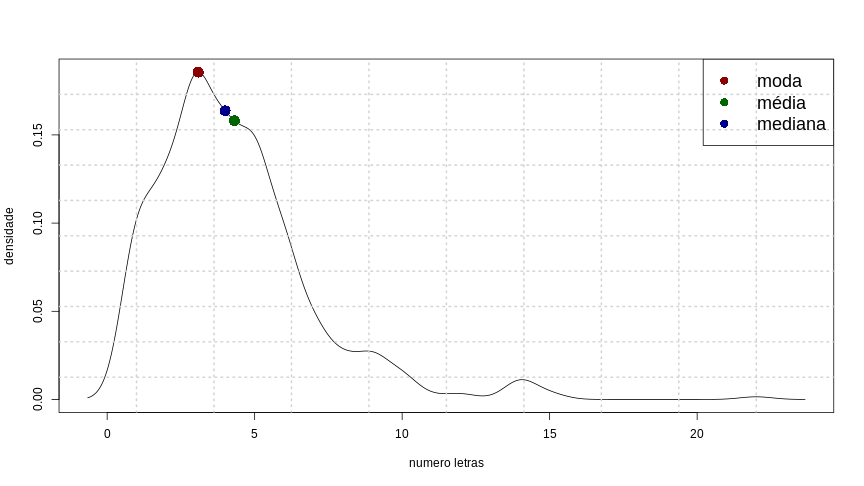
\includegraphics[width=18cm]{densidade_plot.png}};
	\end{tikzpicture}
	Extraindo algumas estatísticas dos dados:
	\begin{lstlisting}
	library(moments)
	vec_n_letras_sel <- data_lemas[data_lemas$cat_gram 
				%in% 'gram',]$nb_letras
	data_density <- density(vec_n_letras_sel,n=4096, 
				bw=1.2*bw.nrd(vec_n_letras_sel))
	idx_max <- which.max(data_density$y)
	moda_data <- data_density$y[idx_max]
	mean_data <- mean(vec_n_letras_sel)
	medi_data <- median(vec_n_letras_sel)
	stdv_data <- sd(vec_n_letras_sel)
	curt_data <- kurtosis(vec_n_letras_sel)
	assi_data <- skewness(vec_n_letras_sel)
	\end{lstlisting}
	\vspace{0.5cm}
	\begin{addmargin}[2cm]{0em}
		\normalsize 
		\begin{verbatim}
		0.1855834
		4.313808
		4
		2.719188
		8.536706
		1.746169
		\end{verbatim}
	\end{addmargin}

\end{frame}
% ------------------------------------------------------------------------
\begin{frame}[t,fragile=singleslide]
\frametitle{Representações bivariadas}
	\begin{tikzpicture}[remember picture,overlay]
	\node[xshift=8cm,yshift=3.75cm,opacity=1.0] at (current page.center) {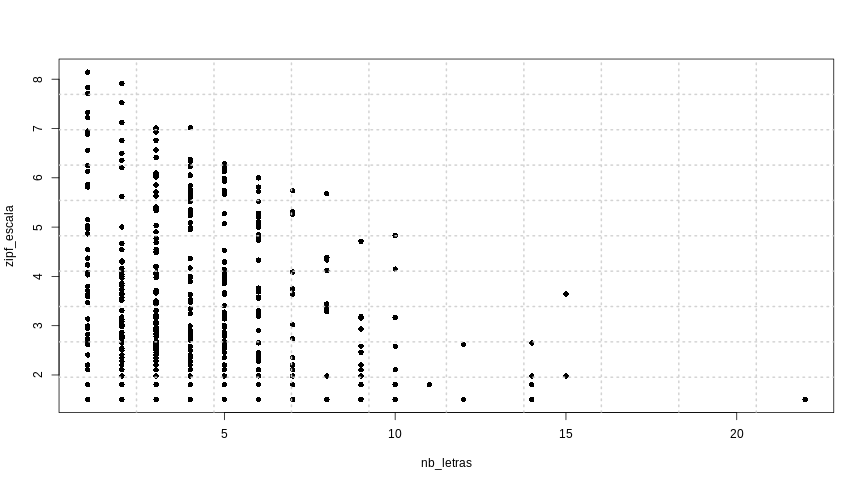
\includegraphics[width=16cm]{scatter_plot_02.png}};
	\end{tikzpicture}
	\vspace{-1.5cm}
	\begin{itemize}
		\item[-] Tabelas de contingência
		\item[-] Gráficos de dispersão
		\item[-] Correlação
		\begin{itemize}
			\item[-] Pearson, Kendall, Spearman
		\end{itemize}
		\item[-] Informação mútua...
	\end{itemize}
	\vspace{0.5cm}
	Extraindo dados de duas variáveis:\\
	\begin{lstlisting}
	vec_X_sel <- data_lemas[data_lemas$cat_gram %in% 'gram',]$nb_letras
	vec_Y_sel <- data_lemas[data_lemas$cat_gram %in% 'gram',]$zipf_escala
	png(file = "../Imagens/scatter_plot_02.png",width = 864, height = 486, bg = "transparent")
	plot(x=vec_X_sel,y=vec_Y_sel,type='p',pch=16,xlab="log10_freq_orto",ylab="zipf_escala")
	grid(10,lwd =2)
	dev.off()
	cor(vec_X_sel,vec_Y_sel)
	\end{lstlisting}
	\vspace{0.5cm}
	\begin{addmargin}[2cm]{0em}
		\normalsize 
		\begin{verbatim}
		-0.2453342 
		\end{verbatim}
	\end{addmargin}
\end{frame}
% ------------------------------------------------------------------------
\begin{frame}[t,fragile=singleslide]
\frametitle{Fim da Estatística Descritiva - Dever de casa}
	\textbf{Exercícios do livro \cite{Agresti2018}:}
	\begin{itemize}
		\item[-] Capítulo 3: 1.1, 1.3, 1.5-1.8, 1.14, 1.16;
	\end{itemize}
	\textbf{Preparação do terreno}
	\begin{itemize}
		\item[-] Reproduzir os exemplos no R-Studio.
	\end{itemize}	
	\vspace{1cm}
	Lembrete:\\
	\textbf{Parâmetros} de populações geralmente são representados por letras gregas, e.g., $\mu$ (média), $\sigma^2$ (variância), $\pi$ (proporção), etc...\\
	\textbf{Estatísticas} são extraídas das amostras e representadas por letras latinas, com ou sem complemento, e.g., $m$, $s^2$, $p$.\\
\end{frame}

% ------------------------------------------------------------------------
\section{Probabilidades}
\begin{frame}[t,fragile=singleslide]
\frametitle{Algumas definições}
	\begin{itemize}
		\item[-] Valor que indica o quão suscetível um evento está de ocorrer.
		\item[-] Proporção de um evento em particular dada uma longa sequência de observações
		\item[-] Bases para o cálculo de probabilidades:
		\begin{itemize}
			\item[-] Axiomas de Kolmogorov
			\item[-] Teorema do limite central (ou central do limite?).
			\item[-] $\sigma$-algebra
			\item[-] lei dos grandes números			
		\end{itemize}
		\item[-] Exemplo do problema de Monty Hall.
	\end{itemize}
	\textbf{Parâmetros}: de populações geralmente são representados por letras gregas, e.g., $\mu$ (média), $\sigma^2$ (variância), $\pi$ (proporção), etc...\\
	\textbf{Estatísticas} são extraídas das amostras e representadas por letras latinas, com ou sem complemento, e.g., $m$, $s^2$, $p$.\\
	\begin{tikzpicture}[remember picture,overlay]
	\node[xshift=10cm,yshift=1.75cm,opacity=1.0] at (current page.center) {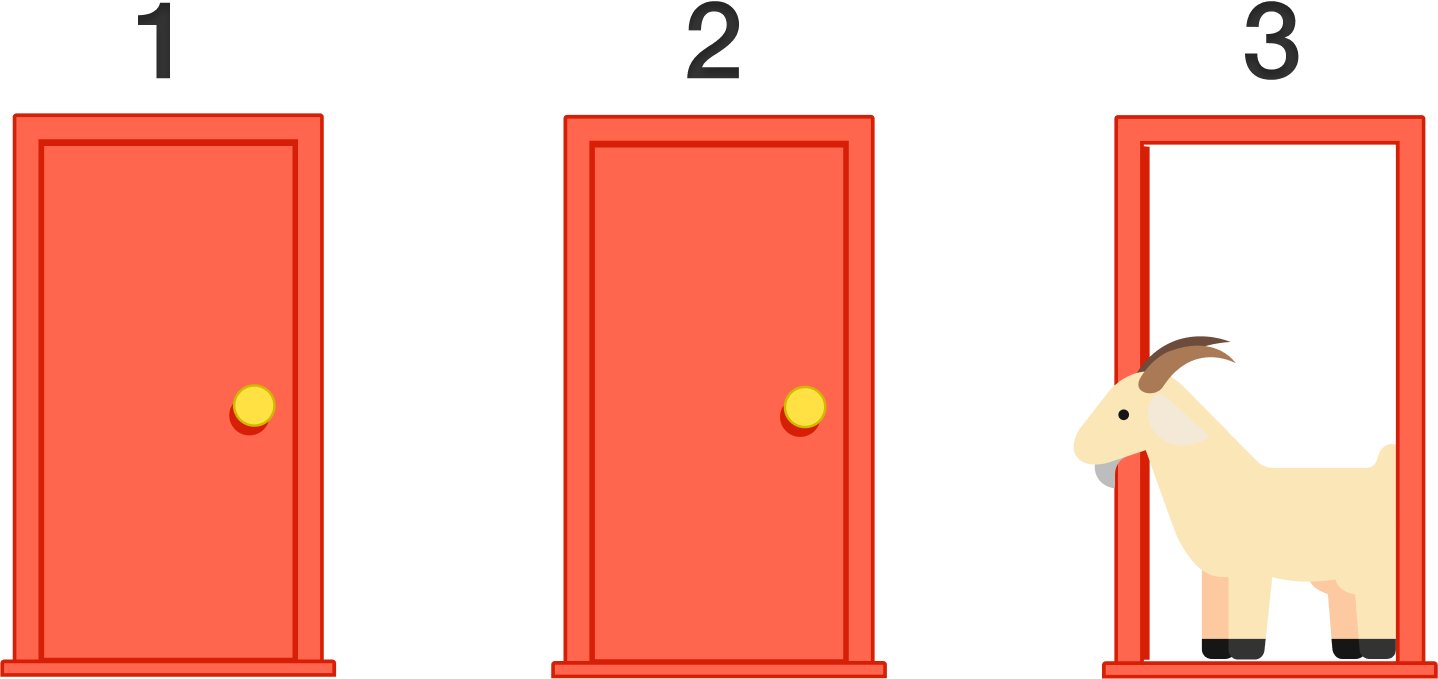
\includegraphics[width=12cm]{monty-hall.png}};
	\end{tikzpicture}
	\vfill
	\lfr{\url{https://brilliant-staff-media.s3-us-west-2.amazonaws.com/tiffany-wang/gWotbuEdYC.png}}
	
\end{frame}

% ------------------------------------------------------------------------
\begin{frame}[t,fragile=singleslide]
\frametitle{Notação e regras básicas I, mais em \citep{Halperin1965}}
	\begin{columns}[T] % align columns
	\begin{column}{.85\textwidth}
		A variável aleatória $x \in X$ significa que um resultado particular (amostra) $x$ pertence $\in$ a variável aleatória/conjunto (população) $X$.\\
		\vspace{0.5cm}
		Se a variável tem seus parâmetros conhecidos, por exemplo, vem de uma distribuição normal (Gaussiana $\mathcal{N}(\mu,\sigma)$) com média igual a 1,7 e desvio padrão de 0,4 podemos escrever $x \in \mathcal{N}(1,7,0,4)$, ou $X \backsim \mathcal{N}(1,7,0,4)$. \\
		\vspace{0.5cm}
		A normal padrão possui média igual a zero e desvio unitário $\mathcal{N}(0,1)$\\		
		\vspace{0.5cm}
		Uma probabilidade de um evento $A$ é definida como $P(\omega:X(\omega) \in A)$ ou simplesmente $P(A)$ (vide nota de rodapé).
		
	\end{column}
	\hfill
	\begin{column}{0.05\textwidth}
	\end{column}		
	\end{columns}
	\vfill
	\lfr{Definições mais formalizadas, como \cite{Halperin1965} e \cite{Wikipedia2017}, sugerem Uma probabilidade qualquer é definida como $\mathbb{P}(A)$ e definir ``P é uma probabilidade''. Mas neste material vou utilizar $P(:)$ por ser mais difundido em livros didáticos.}
	
\end{frame}
% ------------------------------------------------------------------------
\begin{frame}[t,fragile=singleslide]
\frametitle{Notação e regras básicas II, mais em \citep{Halperin1965}}
	\begin{columns}[T] % align columns
		\begin{column}{.85\textwidth}
			Costuma-se fazer referência ao espaço amostral como $\Omega$, assim $P(\Omega) = 1$			
			\vspace{0.5cm}
			Se um evento $A$ tem probabilidade $P(A)$ de ocorrer.\\
			$P(\bar{A}) = 1 - P(A)$ é a probabilidade do evento não ocorrer.\\
			\vspace{0.5cm}
			Dados dois eventos mutualmente independentes $A$ e $B$ (e.g., rodadas diferentes de um lançamento de moeda) e suas probabilidades $P(A)$ e $P(B)$, a probabilidade de ocorrerem:
			\begin{itemize}
				\item[-] $P(A)$ ou $P(B)$ é: $P(A \cup B) = P(A) + P(B)$ (um ou o outro ou os dois)
				\item[-] $P(A)$ e $P(B)$ é: $P(A \cap B) = P(A) \times P(B)$ (concomitantemente)
			\end{itemize} 
			\textbf{Independente}: Dois valores de uma mesma característica categórica, e.g., frequência fundamental grave ou aguda.\\
		\end{column}
		\hfill
		\begin{column}{0.05\textwidth}
		\end{column}		
	\end{columns}
	\vfill

	
\end{frame}
% ------------------------------------------------------------------------
\begin{frame}[t,fragile=singleslide]
\frametitle{Notação e regras básicas III, mais em \citep{Halperin1965}}
\begin{columns}[T] % align columns
	\begin{column}{.85\textwidth}
		Considere dois eventos \textbf{não} mutualmente independentes $A$ e $B$, como valores de características diferentes (e.g., frequência fundamental grave e presença de frênulo lingual) e suas  probabilidade $P(A)$ e $P(B)$. \\
		\vspace{0.5cm}
		A probabilidade  condicional, de ocorrer uma condição dada outra é:
		$P(B|A)$ lê-se $P(B)$ dado $A$\\
		\vspace{0.5cm}
		Neste caso:\\
		$P(A \cap B) = P(A) \times P(B|A)$.\\
		\vspace{0.5cm}
		Teorema de Bayes:\\
		\begin{equation*}
			P(B|A) = \frac{P(B)P(A|B)}{P(A)}
		\end{equation*}
	\end{column}
	\hfill
	\begin{column}{0.05\textwidth}
	\end{column}		
\end{columns}
\vfill

\end{frame}
% ------------------------------------------------------------------------
\begin{frame}[t,fragile=singleslide]
\frametitle{Probabilidades em Diagramas de Venn}
	\begin{tikzpicture}[remember picture,overlay]
	\node[xshift=0cm,yshift=0cm,opacity=1.0] at (current page.center) {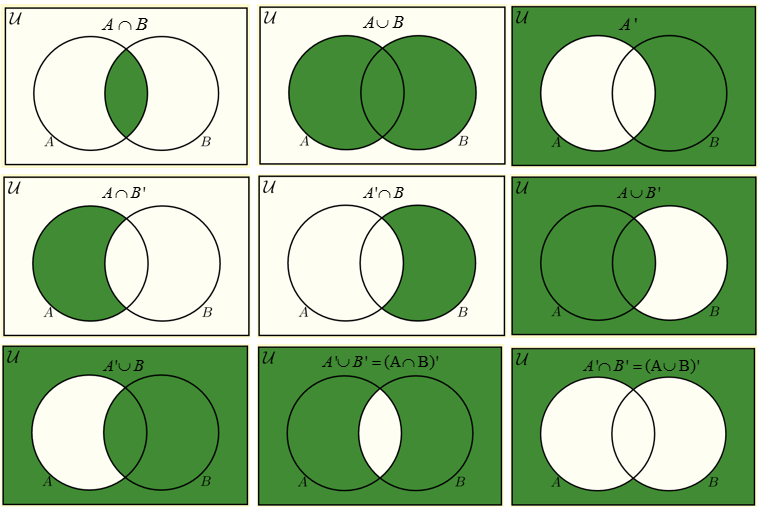
\includegraphics[width=22cm]{venn-diagrams.png}};
	\end{tikzpicture}
	\vfill
	\lfr{\url{https://www.onlinemathlearning.com/image-files/venn-diagrams.png}}

\end{frame}
% ------------------------------------------------------------------------
\begin{frame}[t,fragile=singleslide]
\frametitle{Distribuições}
	Distribuição de uma variável discreta
	\begin{itemize}
		\item[-] $0 \leq P(x) \le 1$.
		\item[-] $\sum P(x) = 1$.
		\item[-] Função massa de probabilidade.
		\item[-] Probabilidade está diretamente em $P(x)$.
	\end{itemize} 
	\vspace{0.5cm}
	Distribuição de uma variável contínua
	\begin{itemize}
		\item[-] $0 \leq P(x) \le 1$. 
		\item[-] $\int\limits_{-\infty}^{\infty} p(x)dx = 1$.
		\item[-] Função densidade de probabilidade $p(x)$.
		\item[-] $P(1 \leq x \leq 3) = \int\limits_{1}^{3} p(x)dx$.
	\end{itemize} 
	\begin{tikzpicture}[remember picture,overlay]
	\node[xshift=8.5cm,yshift=4cm,opacity=1.0] at (current page.center) {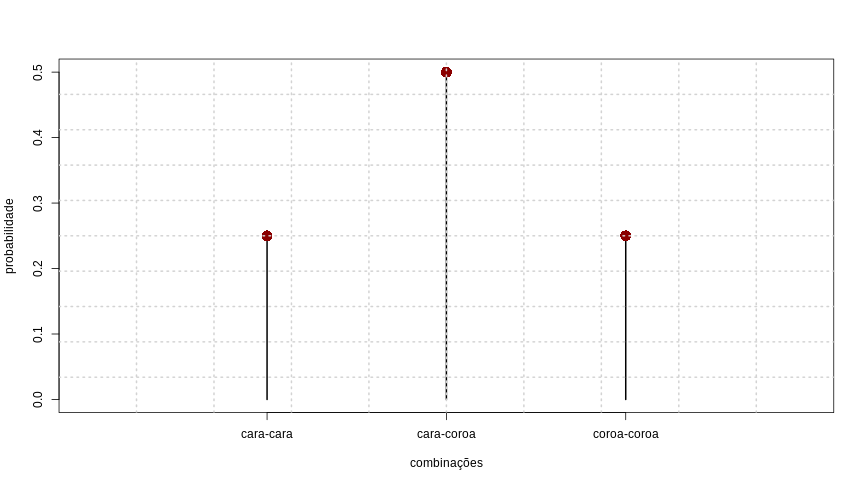
\includegraphics[width=16cm]{prob-discreta-00.png}};
	\end{tikzpicture}
	\begin{tikzpicture}[remember picture,overlay]
	\node[xshift=8.5cm,yshift=-4cm,opacity=1.0] at (current page.center) {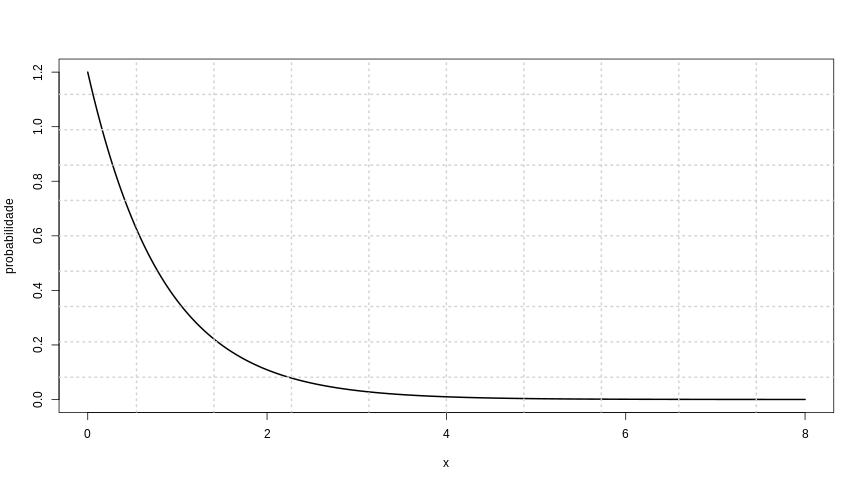
\includegraphics[width=16cm]{prob-continua-00.png}};
	\end{tikzpicture}

	\vfill
\end{frame}
% ------------------------------------------------------------------------
\begin{frame}[t,fragile=singleslide]
\frametitle{Parâmetros - vide \cite{Casella2011}}
	Valor esperado
	\begin{equation*}
		E[x] = \mu  = \sum\limits_{x \in X}xP(x) \quad \text{ou} \quad \mu = \int\limits_{x \in X}xp(x)dx
	\end{equation*}
	Variância
	\begin{equation*}
		E[(x-\mu)]^2 = \sigma^2 = \sum\limits_{x \in X}(x-\mu)^2P(x) \quad \text{ou} \quad  \sigma = \int\limits_{x \in X}(x-\mu)^2p(x)dx
	\end{equation*}
	Momentos estatísticos
	\begin{equation*}
	E[x]^n = \sum\limits_{x \in X}x^nP(x) \quad \text{ou} \quad  \int\limits_{x \in X}x^np(x)dx
	\end{equation*}
	Momentos centrais
	\begin{equation*}
	E[(x-\mu)]^n = \sum\limits_{x \in X}(x-\mu)^nP(x) \quad \text{ou} \quad  \int\limits_{x \in X}(x-\mu)^np(x)dx
	\end{equation*}
\end{frame}
% ------------------------------------------------------------------------
\begin{frame}[t,fragile=singleslide]
\frametitle{Função Normal}
	Padrão com $\mu = 0$ e $\sigma = 1$
	\begin{equation*}
		\mathcal{N}(x|0,1) = \frac{1}{\sqrt{2\pi}}\exp^{-\frac{x^2}{2}}
	\end{equation*}
	Geral, lembrar da regra do $\sigma$
	\begin{equation*}
		\mathcal{N}(x|\mu,\sigma) = \frac{1}{\sqrt{2\pi}\sigma}\exp^{-\frac{(x-\mu)^2}{2\sigma^2}}
	\end{equation*}
	\begin{tikzpicture}[remember picture,overlay]
	\node[xshift=0cm,yshift=-4cm,opacity=1.0] at (current page.center) {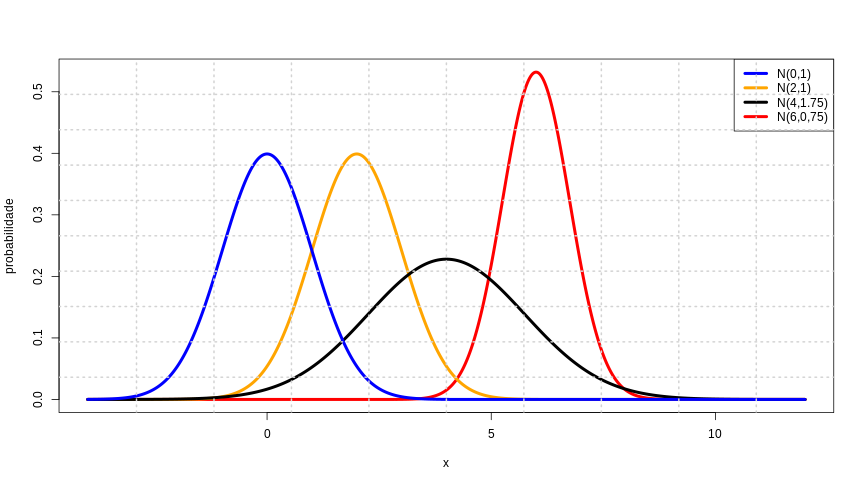
\includegraphics[width=20cm]{prob-normal-00.png}};
	\end{tikzpicture}
\end{frame}
% ------------------------------------------------------------------------
\begin{frame}[t,fragile=singleslide]
\frametitle{Probabilidade acumulada}
	\begin{tikzpicture}[remember picture,overlay]
	\node[xshift=0cm,yshift=3cm,opacity=1.0] at (current page.center) {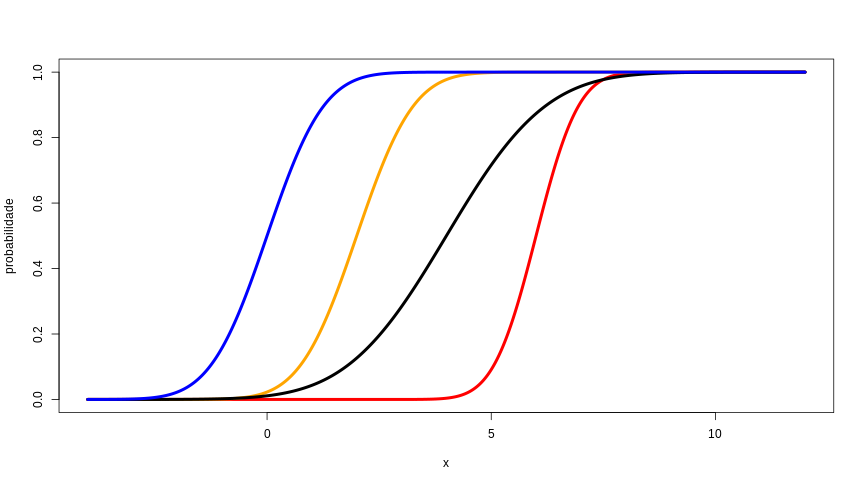
\includegraphics[width=20cm]{prob-normal-acum-00.png}};
	\end{tikzpicture}
	
	\vspace{9.0cm}
	
	Covariância
	\begin{equation*}
	cov(x,y) = E\left[(x-\mu_x)(y-\mu_y) \right]
	\end{equation*}
	Correlação
	\begin{equation*}
	cov(x,y) = E\left[\frac{(x-\mu_x)}{\sigma_x}\frac{(y-\mu_y)}{\sigma_y} \right]
	\end{equation*}
\end{frame}
% ------------------------------------------------------------------------
\begin{frame}[t,fragile=singleslide]
\frametitle{Erro padrão}
	O erro padrão de uma \textbf{estatística} (na maioria das vezes a estimativa de um \textbf{parâmetro}) é o desvio padrão da distribuição amostral de uma estatística.
	
	Erro padrão da média:
	\begin{equation*}
		\sigma_{\bar{x}} = \frac{\sigma}{n}
	\end{equation*}
	
	Em geral, a distribuição amostral da média $\bar{x}$ tende a uma normal independente da distribuição de $X$.
	
\end{frame}
% ------------------------------------------------------------------------
\begin{frame}[t,fragile=singleslide]
\frametitle{Dever de casa}
\end{frame}
% ------------------------------------------------------------------------
\begin{frame}[t,fragile=singleslide]
\frametitle{Dever de casa}
\end{frame}
% ------------------------------------------------------------------------
\begin{frame}[t,fragile=singleslide]
\frametitle{Dever de casa}
\end{frame}
% ------------------------------------------------------------------------
\section[Estimação de Parâmetros]{Estimação de Parâmetros}
\begin{frame}[t,fragile=singleslide]
\frametitle{Dever de casa}
\end{frame}

% ------------------------------------------------------------------------
\begin{frame}[t,fragile=singleslide]
\frametitle{Dever de casa}
\end{frame}
% ------------------------------------------------------------------------
\section[Teste de Significância]{Teste de Significância}
\begin{frame}[t,fragile=singleslide]
\frametitle{Dever de casa}
\end{frame}

% ------------------------------------------------------------------------
\begin{frame}[t,fragile=singleslide]
\frametitle{Dever de casa}
\end{frame}
% ------------------------------------------------------------------------
\section{Comparação de dois grupos}
\begin{frame}[t,fragile=singleslide]
\frametitle{Dever de casa}
\end{frame}

% ------------------------------------------------------------------------
\begin{frame}[t,fragile=singleslide]
\frametitle{Dever de casa}
\end{frame}
% ------------------------------------------------------------------------
\section{Associação de Variáveis Categóricas}
\begin{frame}[t,fragile=singleslide]
\frametitle{Dever de casa}
\end{frame}
% ------------------------------------------------------------------------
\begin{frame}[t,fragile=singleslide]
\frametitle{Dever de casa}
\end{frame}
% ------------------------------------------------------------------------
\section{Regressão Linear e Correlação}
\begin{frame}[t,fragile=singleslide]
\frametitle{Dever de casa}
\end{frame}
% ------------------------------------------------------------------------
\begin{frame}[t,fragile=singleslide]
\frametitle{Dever de casa}
\end{frame}
% ------------------------------------------------------------------------
\section{Relação Multivariável}
\begin{frame}[t,fragile=singleslide]
\frametitle{Dever de casa}
\end{frame}
% ------------------------------------------------------------------------
\begin{frame}[t,fragile=singleslide]
\frametitle{Dever de casa}
\end{frame}
% ------------------------------------------------------------------------
\section{Regressão Múltipla e Correlação}
\begin{frame}[t,fragile=singleslide]
\frametitle{Dever de casa}
\end{frame}
% ------------------------------------------------------------------------
\begin{frame}[t,fragile=singleslide]
\frametitle{Dever de casa}
\end{frame}
% ------------------------------------------------------------------------
\section{Análise de Variância - ANOVA}
\begin{frame}[t,fragile=singleslide]
\frametitle{Dever de casa}
\end{frame}
% ------------------------------------------------------------------------
\begin{frame}[t,fragile=singleslide]
\frametitle{Dever de casa}
\end{frame}
% ------------------------------------------------------------------------
\section{Preditores Quantitativos e Categóricos}
\begin{frame}[t,fragile=singleslide]
\frametitle{Dever de casa}
\end{frame}
% ------------------------------------------------------------------------
\begin{frame}[t,fragile=singleslide]
\frametitle{Dever de casa}
\end{frame}
% ------------------------------------------------------------------------
\section{Modelos com Regressão Múltipla}
\begin{frame}[t,fragile=singleslide]
\frametitle{Dever de casa}
\end{frame}
% ------------------------------------------------------------------------
\begin{frame}[t,fragile=singleslide]
\frametitle{Dever de casa}
\end{frame}
% ------------------------------------------------------------------------
\section{Regressão Logística}
\begin{frame}[t,fragile=singleslide]
\frametitle{Dever de casa}
\end{frame}
% ------------------------------------------------------------------------
\begin{frame}[t,fragile=singleslide]
\frametitle{Dever de casa}
\end{frame}
% ------------------------------------------------------------------------
\section{Introdução a métodos aprofundados}
\begin{frame}[t,fragile=singleslide]
\frametitle{Dever de casa}
\end{frame}
% ------------------------------------------------------------------------
\begin{frame}[t,fragile=singleslide]
\frametitle{Dever de casa}
\end{frame}
% ------------------------------------------------------------------------
\section{Encerramento}
\begin{frame}[fragile=singleslide]
\frametitle{Sobre este material}%{Condições de uso e referência}

	Esta obra está licenciada sob a licença \textit{Creative Commons} CC BY-NC-SA 4.0 (mais detalhes neste \href{http://creativecommons.org/licenses/by-nc-sa/4.0/}{\textit{link}})\\
%	
	\flushleft
	Favor fazer referência a este trabalho como:\linebreak
	
	Silva, A. P. (2022), \textit{Notas de Aulas de Estatística para Linguística}. Online: {\url{https://github.com/adelinocpp/estatistica-para-linguistica}}
	\linebreak
	\begin{addmargin}[2cm]{0em}
		\normalsize 
		\begin{verbatim}
		@Misc{Silva2022,
		title={Notas de Aulas de Notas de Aulas de Estatística para Linguística},
		author={Adelino Pinheiro Silva},
		howPublished={\url{https://github.com/adelinocpp/estatistica-para-linguistica}},
		year={2022},
		note={Version 1.0; Creative Commons BY-NC-SA 4.0.},
		}
		\end{verbatim}
	\end{addmargin}
	\vfill
	\begin{tikzpicture} [remember picture,overlay]
		\node[anchor=south,yshift=0pt] at (current page.south){ 
\includegraphics[width=.1\textwidth]{00BAS_CCsomerights.png}};
	\end{tikzpicture}
\end{frame} 


% =======================================================================
\section{Referências}

\begin{frame}[allowframebreaks, t]{Referências}
	\bibliographystyle{apalike}
    \bibliography{EST_Aula_01_v00}
\end{frame}
% ======================================================================= 

\end{document}
